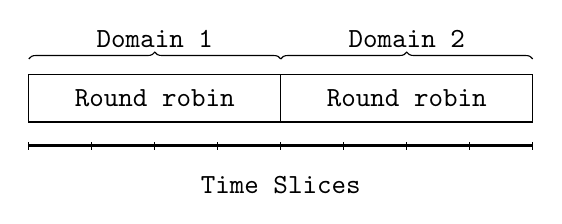
\begin{tikzpicture}[font=\ttfamily]

    % Style for general text nodes
    \tikzset{lbl/.style={inner sep=1pt, align=center}}

    % Define vertical coordinates for rows and labels
    \def\barheight{0.6} % Height of each bar
    \def\vtopprio{1.5}   % Vertical center of the top bar row
    \def\ytimeline{\vtopprio - \barheight} % Vertical position of the minor frames timeline

    % Define standard tick positions
    \def\timeslice{0.8}

    % --- Bar Rows (drawn inside outlines) ---

    % First domain
    \path[draw, decorate, decoration=brace] (0, \vtopprio + 0.5) -- (\timeslice * 4, \vtopprio + 0.5) node[lbl, midway, above, yshift=0.3em]{Domain 1};
    \draw (0, \vtopprio-\barheight/2) rectangle (\timeslice*4, \vtopprio+\barheight/2) 
      node[lbl, midway]{Round robin};

    % Second domain
    \path[draw, decorate, decoration=brace] (\timeslice * 4, \vtopprio + 0.5) -- (\timeslice * 8, \vtopprio + 0.5) node[lbl, midway, above, yshift=0.3em]{Domain 2};
    \draw (\timeslice*4, \vtopprio-\barheight/2) rectangle (\timeslice*8, \vtopprio+\barheight/2) 
      node[lbl, midway]{Round robin};

    % Main timeline axis
    \draw[thick] (0, \ytimeline) -- (8*\timeslice, \ytimeline);

    % Intermediate ticks (not all but to give structure)
    \foreach \x in {0, ..., 8} {
         \draw (\x*\timeslice, \ytimeline-0.05) -- (\x*\timeslice, \ytimeline+0.05);
    }

    % Central label below the timeline
    \node[lbl] at ( { 4 * \timeslice }, \ytimeline-0.5 ) {Time Slices};

\end{tikzpicture}

